
\documentclass[a4paper,11pt]{article}
\usepackage[a4paper, margin=8em]{geometry}

% usa i pacchetti per la scrittura in italiano
\usepackage[french,italian]{babel}
\usepackage[T1]{fontenc}
\usepackage[utf8]{inputenc}
\frenchspacing 

% usa i pacchetti per la formattazione matematica
\usepackage{amsmath, amssymb, amsthm, amsfonts}

% usa altri pacchetti
\usepackage{gensymb}
\usepackage{hyperref}
\usepackage{standalone}

% imposta il titolo
\title{Appunti Fondamenti di Automatica}
\author{Luca Seggiani}
\date{2025}

% disegni
\usepackage{pgfplots}
\pgfplotsset{width=10cm,compat=1.9}

% imposta lo stile
% usa helvetica
\usepackage[scaled]{helvet}
% usa palatino
\usepackage{palatino}
% usa un font monospazio guardabile
\usepackage{lmodern}

% tikz in sans
\tikzset{every picture/.style={/utils/exec={\sffamily}}}

\renewcommand{\rmdefault}{ppl}
\renewcommand{\sfdefault}{phv}
\renewcommand{\ttdefault}{lmtt}

% circuiti
\usepackage{circuitikz}
\usetikzlibrary{babel}

% disponi il titolo
\makeatletter
\renewcommand{\maketitle} {
	\begin{center} 
		\begin{minipage}[t]{.8\textwidth}
			\textsf{\huge\bfseries \@title} 
		\end{minipage}%
		\begin{minipage}[t]{.2\textwidth}
			\raggedleft \vspace{-1.65em}
			\textsf{\small \@author} \vfill
			\textsf{\small \@date}
		\end{minipage}
		\par
	\end{center}

	\thispagestyle{empty}
	\pagestyle{fancy}
}
\makeatother

% disponi teoremi
\usepackage{tcolorbox}
\newtcolorbox[auto counter, number within=section]{theorem}[2][]{%
	colback=blue!10, 
	colframe=blue!40!black, 
	sharp corners=northwest,
	fonttitle=\sffamily\bfseries, 
	title=Teorema~\thetcbcounter: #2, 
	#1
}

% disponi definizioni
\newtcolorbox[auto counter, number within=section]{definition}[2][]{%
	colback=red!10,
	colframe=red!40!black,
	sharp corners=northwest,
	fonttitle=\sffamily\bfseries,
	title=Definizione~\thetcbcounter: #2,
	#1
}

% disponi problemi
\newtcolorbox[auto counter, number within=section]{problem}[2][]{%
	colback=green!10,
	colframe=green!40!black,
	sharp corners=northwest,
	fonttitle=\sffamily\bfseries,
	title=Problema~\thetcbcounter: #2,
	#1
}

% disponi codice
\usepackage{listings}
\usepackage[table]{xcolor}

\lstdefinestyle{codestyle}{
	backgroundcolor=\color{black!5}, 
	commentstyle=\color{codegreen},
	keywordstyle=\bfseries\color{magenta},
	numberstyle=\sffamily\tiny\color{black!60},
	stringstyle=\color{green!50!black},
	basicstyle=\ttfamily\footnotesize,
	breakatwhitespace=false,         
	breaklines=true,                 
	captionpos=b,                    
	keepspaces=true,                 
	numbers=left,                    
	numbersep=5pt,                  
	showspaces=false,                
	showstringspaces=false,
	showtabs=false,                  
	tabsize=2
}

\lstdefinestyle{shellstyle}{
	backgroundcolor=\color{black!5}, 
	basicstyle=\ttfamily\footnotesize\color{black}, 
	commentstyle=\color{black}, 
	keywordstyle=\color{black},
	numberstyle=\color{black!5},
	stringstyle=\color{black}, 
	showspaces=false,
	showstringspaces=false, 
	showtabs=false, 
	tabsize=2, 
	numbers=none, 
	breaklines=true
}

\lstdefinelanguage{javascript}{
	keywords={typeof, new, true, false, catch, function, return, null, catch, switch, var, if, in, while, do, else, case, break},
	keywordstyle=\color{blue}\bfseries,
	ndkeywords={class, export, boolean, throw, implements, import, this},
	ndkeywordstyle=\color{darkgray}\bfseries,
	identifierstyle=\color{black},
	sensitive=false,
	comment=[l]{//},
	morecomment=[s]{/*}{*/},
	commentstyle=\color{purple}\ttfamily,
	stringstyle=\color{red}\ttfamily,
	morestring=[b]',
	morestring=[b]"
}

% disponi sezioni
\usepackage{titlesec}

\titleformat{\section}
{\sffamily\Large\bfseries} 
{\thesection}{1em}{} 
\titleformat{\subsection}
{\sffamily\large\bfseries}   
{\thesubsection}{1em}{} 
\titleformat{\subsubsection}
{\sffamily\normalsize\bfseries} 
{\thesubsubsection}{1em}{}

% disponi alberi
\usepackage{forest}

\forestset{
	rectstyle/.style={
		for tree={rectangle,draw,font=\large\sffamily}
	},
	roundstyle/.style={
		for tree={circle,draw,font=\large}
	}
}

% disponi algoritmi
\usepackage{algorithm}
\usepackage{algorithmic}
\makeatletter
\renewcommand{\ALG@name}{Algoritmo}
\makeatother

% disponi numeri di pagina
\usepackage{fancyhdr}
\fancyhf{} 
\fancyfoot[L]{\sffamily{\thepage}}

\makeatletter
\fancyhead[L]{\raisebox{1ex}[0pt][0pt]{\sffamily{\@title \ \@date}}} 
\fancyhead[R]{\raisebox{1ex}[0pt][0pt]{\sffamily{\@author}}}
\makeatother

\begin{document}

% sezione (data)
\section{Lezione del 16-04-25}

% stili pagina
\thispagestyle{empty}
\pagestyle{fancy}

% testo
Riprendiamo il discorso sul luogo delle radici, con maggiore attenzione su come \textit{tarare} (ottenere informazioni riguardo al modulo) i punti $s$.

\subsubsection{Taratura del luogo delle radici}
Abbiamo visto nella scorsa lezione come applicando la \textit{condizione di fase} possiamo tracciare tutto il luogo delle radici, diretto ed inverso.
Abbiamo poi introdotto come l'altra condizione, la \textit{condizione di modulo}, può essere usata per ottenere il modulo corrispondente ad un punto $s_i$ che già sappiamo appartenere al luogo delle radici.

Questa era quindi la condizione, che valutiamo nel punto $s_i$:
$$
\left| \frac{n(s)}{d(s)} \right| = \frac{1}{|K|} \xrightarrow{s_i} |K| \big|_{s = s_i} = \left| \frac{d(s_i)}{n(s_i)} \right|
$$

Riprendiamo l'esempio della scorsa lezione, che era:
$$
K \cdot G(s) = \frac{K}{s (s + 1)}
$$

Avremo quindi, applicando la condizione di modulo:
$$
|K| \big|_{s = s_i} = \frac{|s_i (s_i + 1)|}{|1|}
$$

Prendiamo ad esempio il punto che sta all'intersezione fra i due rami che avevamo individuato nel luogo diretto, cioè $s_i = -\frac{1}{2}$.
In questo caso avremo che il modulo di $K$ è:
$$
|K| \Big|_{s_i = -\frac{1}{2}} = \frac{\left|-\frac{1}{2} (-\frac{1}{2} + 1)\right|}{|1|} = \frac{1}{4}
$$

\subsection{Luogo delle radici complesse e coniugate}
Veniamo quindi a come tracciare i luoghi delle radici di sistemi del second'ordine.
Prendiamo quindi un nuovo esempio, che è la classica forma di Evans al secondo grado:
$$
G(s) = \frac{\omega_0^2}{s^2 + 2 \xi \omega_0 s + \omega_0 ^2}
$$
Le radici di questa sono note e valgono:
$$
p_{1, 2} = -\xi \omega_0 \pm \omega_0 j \sqrt{1 - \xi^2}
$$

\subsubsection{Valutazione di frequenza e smorzamento}

Vediamo quali informazioni sul sistema possiamo ottenere osservando le radici.

Prendendo quindi un punto all'origine nel piano di Gauss del luogo delle radici, e quindi l'angolo $\theta$ che la congiungente del punto e la radice a parte immaginaria positiva forma con l'asse immaginario, potremo dire:
$$
\omega_0 \sin(\theta) = \xi \omega_0 \implies \theta = \sin^{-1} (\xi) 
$$
cioè l'angolo $\theta$ va più o meno come lo smorzamento.

Di contro, considerando smorzamente fisso, si ha che la distanza dall'origine equivale alla frequenza naturale.
Infatti avremo che:
$$
\sqrt{ \xi^2 \omega_0^2 + \omega_0^2 (1 - \xi^2) } = \omega_0
$$

Riassumendo, quindi, si ha che:
\begin{itemize}
	\item $\xi = 0$: (\textit{smorzamento nullo}) i poli sono sull'asse immaginario;
	\item $\xi = 1$: (\textit{smorzamento perfetto})  i poli sono sul'asse reale e coincidenti;
	\item $0 < \xi < 1$: (\textit{sistema sottosmorzato}) i poli sono sulla semicirconferenza sinistra (uno in $\mathbb{C}^+$, l'altro in $\mathbb{C}^-$) di raggio $\omega_0$ centrata sull'origine.
	\item Il modulo delle radici corrisponde alla frequenza naturale $\omega_0$.
\end{itemize}

\subsubsection{Linee costanti}
Esistono diverse linee costanti che possiamo percorrere (cioè su cui possiamo posizionare i poli) in modo da mantenere certe caratteristiche del sistema costanti:
\begin{itemize}
	\item 
		Abbiamo quindi che percorrendo una retta passante per l'origine nella direzione negativa dell'asse complesso si ottiene una cosiddetta \textbf{linea di smorzamento costante}, cioè un insieme di regioni dove lo smorzamento resta costante e cambia invece (con l'aumentare della distanza dall'origine) la frequenza naturale. 

		Vediamo ad esempio il seguente grafico, dove a sinistra si mostrano le linee di smorzamento costante, e a sinistra le risposte all'impulso di alcuni dei sistemi che descrivono:
		\begin{center}
			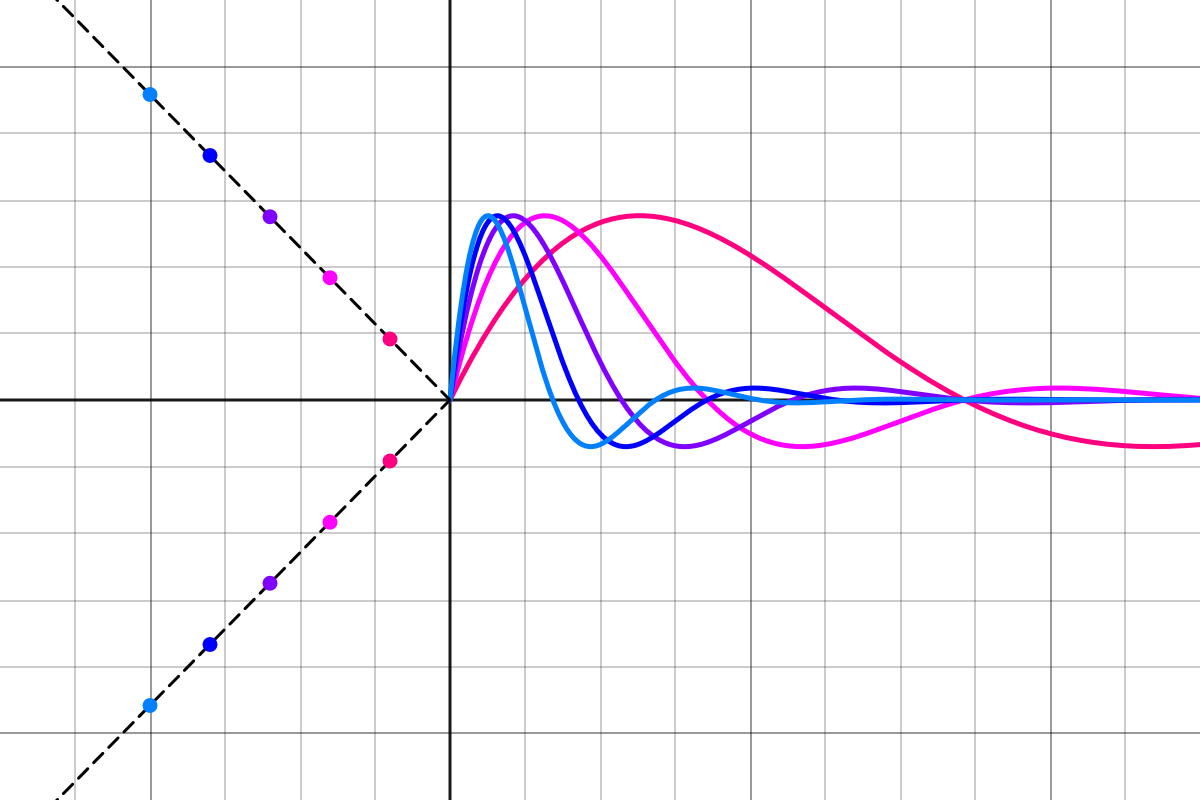
\includegraphics[scale=0.28]{../figures/fixed_damping.png}
		\end{center}
	\item
		Per mantenere costante il tempo di assestamento, invece, basta mantenere la componente reale dei poli costante, ergo si crea una cosiddetta \textbf{linea di tempo di assestamento costante} parallela all'asse immaginario. 

		\newpage

		Il grafico del tipo precedente per questa situazione è:
		\begin{center}
			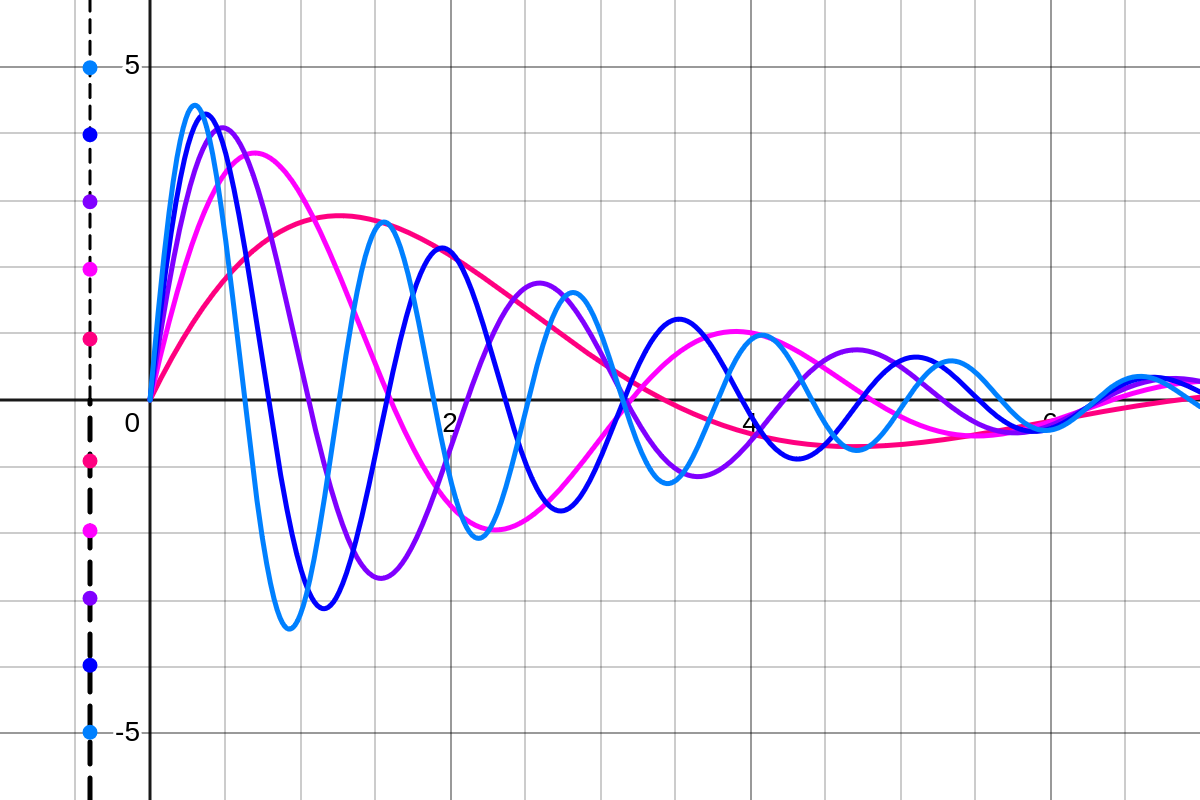
\includegraphics[scale=0.28]{../figures/fixed_time.png}
		\end{center}
	\item
		Per mantenere costante la pulsazione prendiamo circonferenze centrate sull'origine di raggio crescente, cioè cerchiamo una \textbf{circonferenza di pulsazione costante}.
		
		Il grafico del tipo precedente per questa situazione è:
		\begin{center}
			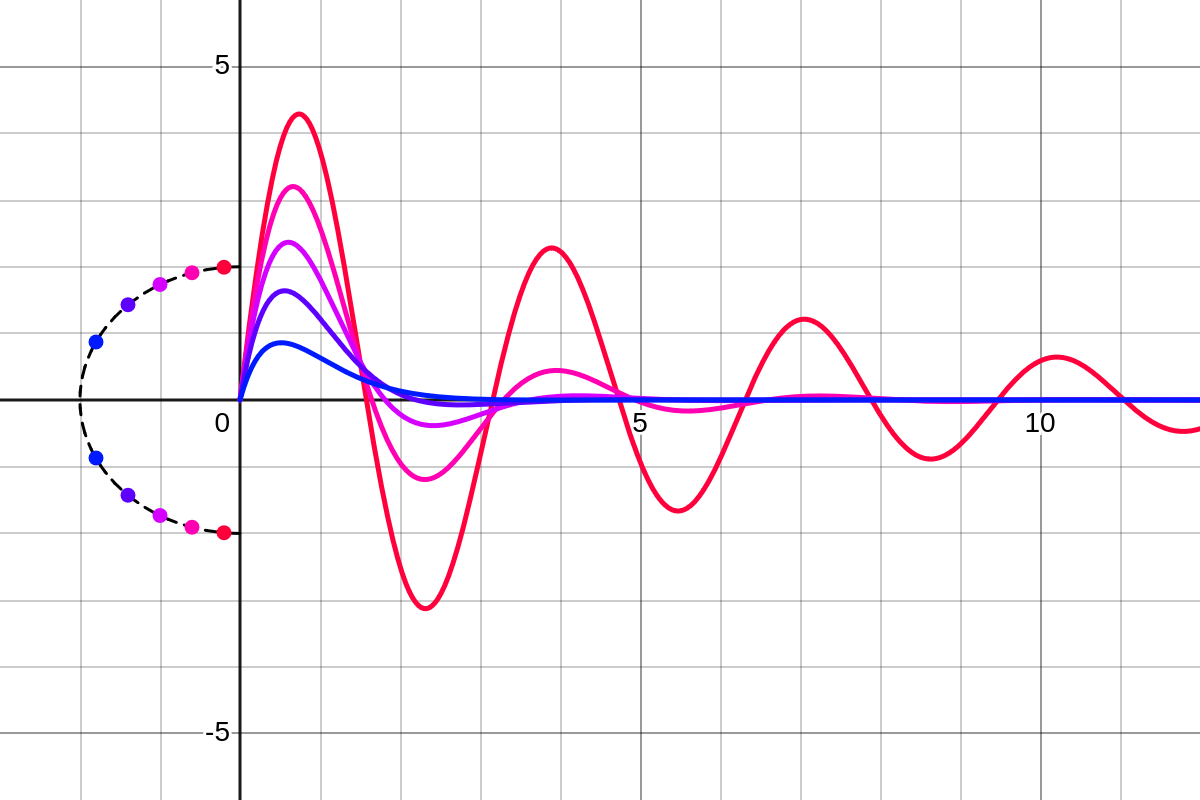
\includegraphics[scale=0.28]{../figures/fixed_pulse.png}
		\end{center}
\end{itemize}

\subsubsection{Regioni di vincolo}
Abbiamo parlato finora dei soli poli: vediamo di reintrodurre il sistema con controllore ($K$). 

Intanto possiamo vedere alcuni vincoli di progetto che potremmo avere sul comportamento desiderato:
\begin{itemize}
	\item 
		Potremmo volere che lo \textbf{smorzamento} che otterremo non sia mai minore di un certo valore. Saremo vincolati ad un cono di angolo $\theta$ con l'asse immaginario, che possiamo individuare sul piano di Argand-Gauss:
		\begin{center}
			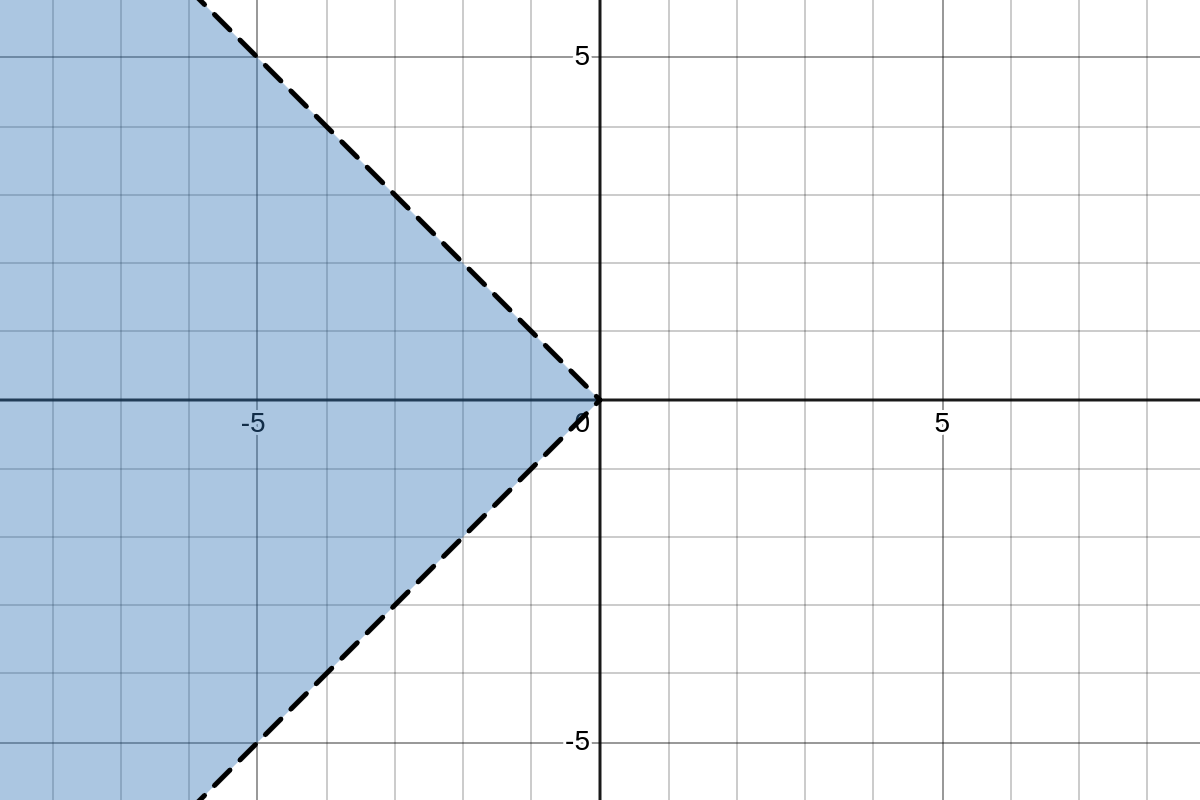
\includegraphics[scale=0.28]{../figures/fixed_damping_region.png}
		\end{center}

	\item
		Se volessimo invece \textbf{tempo di assestamento} sotto una certa soglia, vorremo trovarci a sinistra di una linea di tempo di assestamento costante, quindi in una regione di piano che il seguente aspetto:
		\begin{center}
			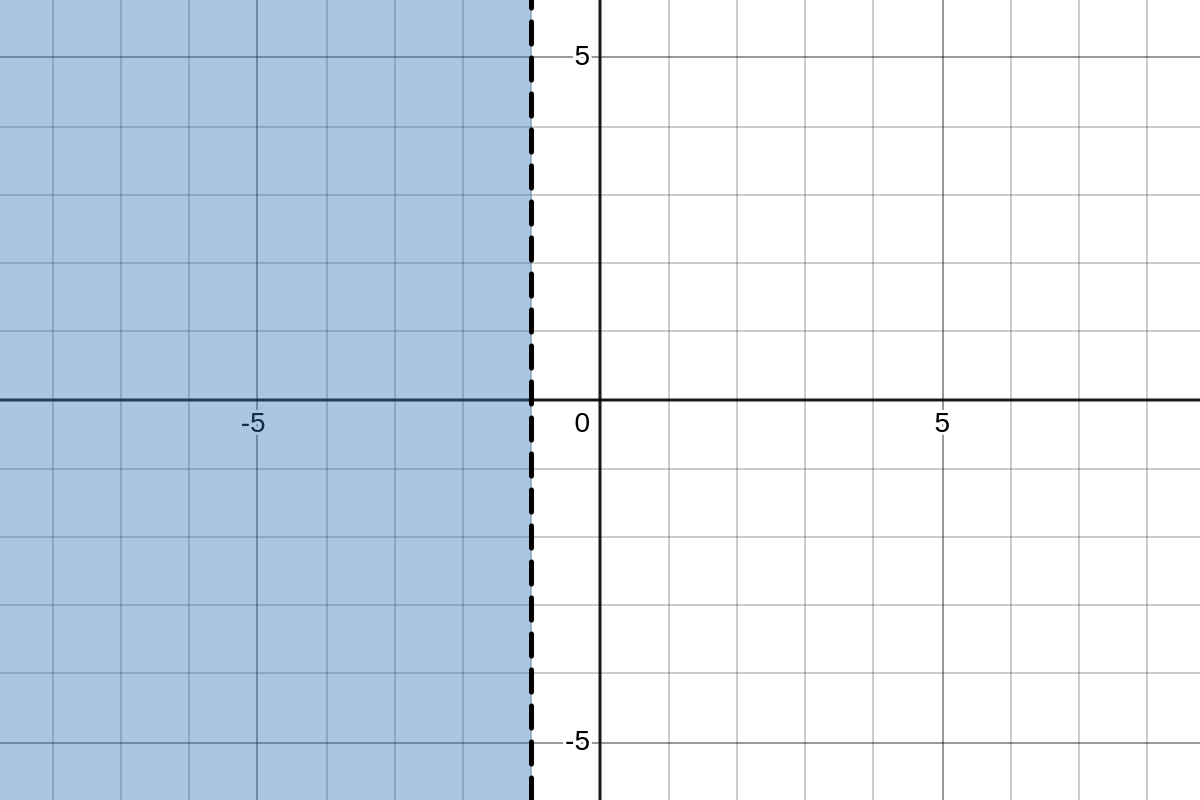
\includegraphics[scale=0.28]{../figures/fixed_time_region.png}
		\end{center}

	\item
		Infine potremmo voler vincolare la pulsazione naturale.
		In questo caso, direttamente dalla corrispondenza fra modulo e pulsazione naturale, ci vorremmo restiringere, ad esempio se si vuole pulsazione \textit{maggiore} (\textit{minore}) di una certa soglia, alla regione \textit{esterna} (\textit{interna}) ad una certa circonferenza di raggio equivalente alla soglia.
		
		\newpage

		Sul grafico:
		\begin{center}
			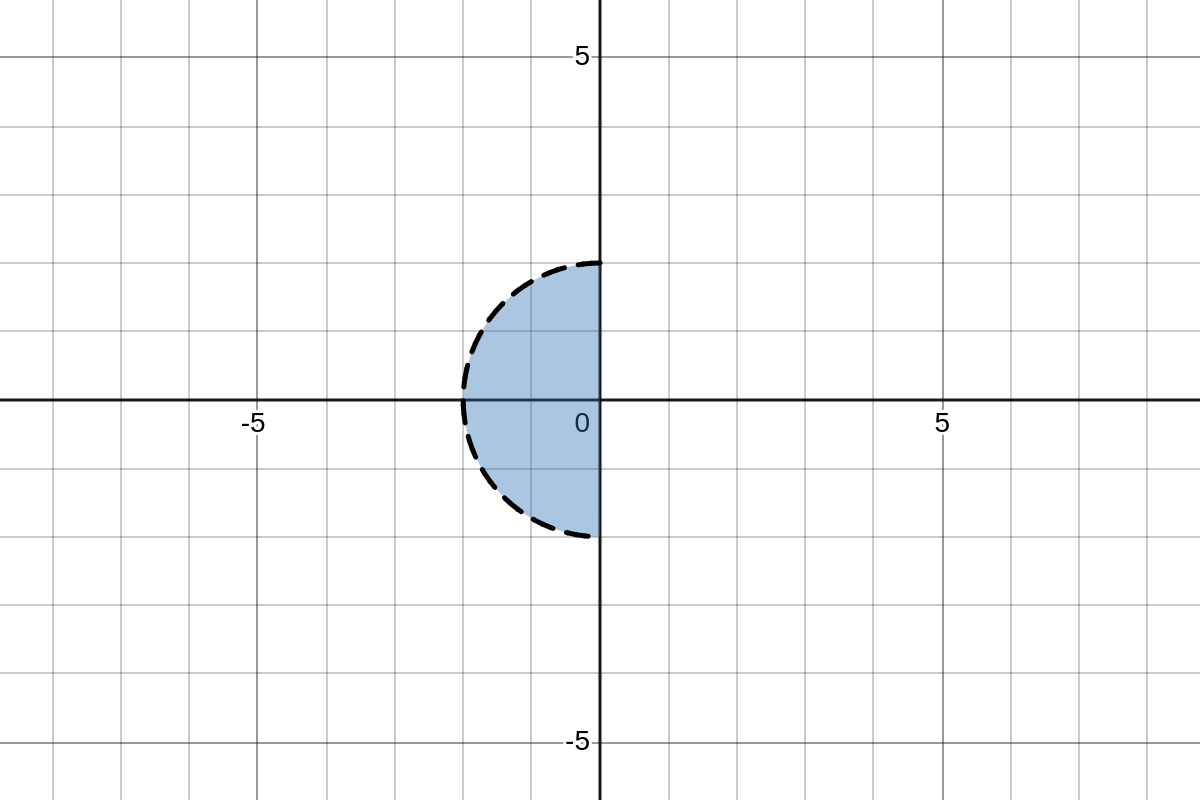
\includegraphics[scale=0.28]{../figures/fixed_pulse_region.png}
		\end{center}
\end{itemize}

L'insieme dei punti che rispettano tutti i vincoli si ha, a questo punto, semplicemente prendendo l'intersezione delle regioni individuate da ogni vincolo.

\subsubsection{Regole di tracciamento 2}
Vediamo quindi altre regole di tracciamento.

\begin{enumerate}
	\item[5.] La regola (5) riguarda le \textit{sovrapposizioni} di rami.
		In particolare, si ha che i rami non si sovrappongono mai, se non in punti singolari detti \textbf{punti multipli}, in quanto rappresentano \textit{radici multiple} del polinomio caratteristico.

		In un punto multiplo la radice multipla $s_i$ è soluzione di:
		\[
			\begin{cases}
				d(s_i) + Kn(s_i) = 0 \\
				d'(s_i) + K n'(s_i) = 0
			\end{cases}
		\]
		cioè dell'equazione caratteristica e della sua derivata.

		Inoltre, si nota che:
		$$
		\sum_{i = 1}^n \frac{1}{s_i - p_i} = \sum_{i = 1}^m \frac{1}{s_i - z_i}
		$$

		\par\medskip
		\noindent
		\textbf{\sffamily{Esempio}}

		Avevamo già visto questa situazione nel primo esempio di tracciamento, cioè:
		$$
		K \cdot G(s) = \frac{K}{s(s+1)}
		$$

		Vediamo infatti che risolvendo:
		$$
		\sum_{i = 1}^n \frac{1}{s - p_i} = \sum_{i = 1}^m \frac{1}{s - z_i}
		\implies \frac{1}{s} + \frac{1}{s + 1} = 0
		$$
		si ottiene la soluzione:
		$$
		s_i = -\frac{1}{2}
		$$
		che avevamo visto era esattamente un punto di intersezione fra rami (in particolare quello reale e immaginario nel luogo diretto).

	\item[6.] La regola (6) si concentra sul \textit{comportamento asintotico}, cioè su cosa accade per $K \rightarrow +\infty$.
		Avevamo anticipato che in questo caso i poli andavano al \textit{finito} (cioè agli zeri della funzione a ciclo aperto) o ad \textit{infinito}.
		Per quanto riguardava i poli ad infinito, avevamo detto che questi erano $n - m$ (cioè quelli che non andavano in zeri in ciclo aperto).
		Chiamiamo questo valore $v = n - m$, o \textit{differenza poli-zeri}.

		Avevamo dalla condizione di fase, cioè dalla regola (2), che i punti che appartengono al luogo delle radici sono quelli che rispettano:
		\[
			\begin{cases}
				\angle n(s) - \angle d(s) = -\pi \pm 2 h \pi, \quad K > 0 \\
				\angle n(s) - \angle d(s) = \pm 2 h \pi, \quad K < 0
			\end{cases}
		\]
		e cioè per cui la somma degli angoli agli zeri $\theta_i$ meno la somma degli angoli ai poli $\phi_i$ vale $-\pi$ per il luogo diretto, e $0$ per il luogo indiretto.
		Quando facciamo tendere $K$ ad infinito, si ha che gli angoli per tutti i poli e zeri diventano simili, cioè:
		$$
		\phi_i \approx \theta_i \approx \phi_\infty
		$$
		per cui potremo approssimare:
		$$
		\angle n(s) - \angle d(s) \approx \phi_{\infty} (m - n) = -\pi \pm 2 h \pi
		$$
		da cui la regola (nell'esempio per il luogo diretto).
		Notiamo che preferiamo usare $n - m$ invece di $m - n$ in quanto corrisponde direttamente con $v$, ma il risultato non cambia in quanto la condizione di fase funziona scambiando i segni a destra (se si ruota di $360^\circ$ su un cerchio si torna da dove si è partiti).

		Nota la differenza poli-zeri potremo quindi dire che:
		\begin{itemize}
			\item Esiste un \textbf{centro degli asintoti}, cioè il punto da cui iniziamo a tracciare gli asintoti, che sta sempre sull'asse reale ed è:
				$$
				\sigma = \frac{ \sum_{i = 1}^n p_i - \sum_{i = 1}^m z_i }{v}
				$$

			\item Gli asintoti dividono quindi il piano di Argand-Gauss in sezioni equiangole, cioè si hano gli \textbf{angoli di asintoto}:
				\[
					\phi_\text{asintoto} =
					\begin{cases}
						\frac{-\pi \pm 2 h \pi}{v}, \quad K > 0 \\
						\frac{2 h \pi}{v}, \quad K < 0 \\
					\end{cases}
				\]
		\end{itemize}

		\par\medskip
		\noindent
		\textbf{\sffamily{Esempio 1}}

		Vediamo la funzione di trasferimento di esempio:
		$$
		G(s) = \frac{1}{(s + 1)^3}
		$$
		in questo caso avremo il centro degli asintoti:
		$$
		\sigma = \frac{-1 -1 -1}{3} = -1
		$$
		e gli angoli di asintoto, rispettivamente per il luogo diretto e inverso:
		$$
		\phi_{asintoto} = \left\{ 60^\circ, 180^\circ, 300^\circ \right\}, \quad K > 0
		$$
		$$
		\phi_{asintoto} = \left\{ 0^\circ, 120^\circ, 240^\circ \right\}, \quad K < 0
		$$
		Notiamo che questi angoli non sono stati calcolati usando la formula, ma semplicemente notando di dover dividere, per $v = 3$, il piano di Argand-Gauss in regioni equiangole di angolo $120^\circ$.

	Sul grafico, questo sarà:
	\begin{center}
		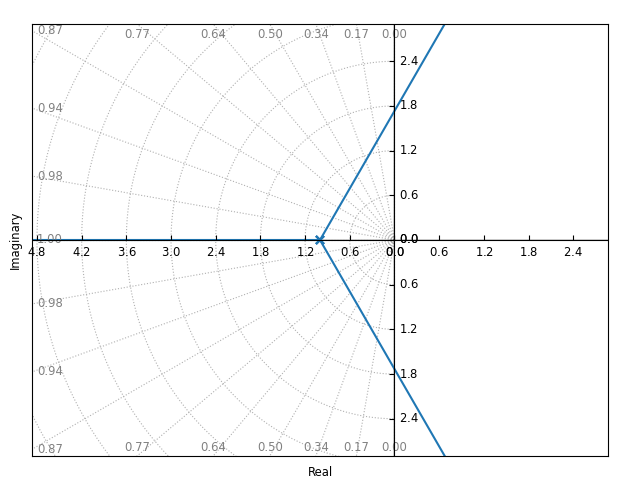
\includegraphics[scale=0.8]{../figures/rlocus/1331.png}
	\end{center}

		\par\medskip
		\noindent
		\textbf{\sffamily{Esempio 2}}

		Vediamo un'altro esempio, attraverso la funzione di trasferimento:
		$$
		G(s) = \frac{1}{s(s + 1)(s + 2)}
		$$
		In questo caso l'equazione caratteristica sarà:
		$$
		1 + K \cdot G(s) = s ( s + 1) ( s + 2) + K = s^3 + 3s^2 + 2s + K = 0
		$$

		Potrebbe interessarci valutare la stablità.
		In questo caso potremmo sfruttare il \textit{criterio di Routh}:
		\begin{table}[H]
			\center 
			\begin{tabular} { c | c c}
				$3$ & $1$ & $2$ \\
				$2$ & $3$ & $K$ \\
				$1$ & $\frac{6 - K}{3}$ & $0$ \\
				$0$ & $K$
			\end{tabular}
		\end{table}
		da cui le $K$ critiche $K_{CR1} = 0$ e $K_{CR2} = 6$, e quindi sistema stabile per $0 < K < 6$.

		Proseguiamo col tracciamento.
		Avremo che i poli sono $p_1 = -2$, $p_2 = -1$ e $p_3 = 0$
		Dalla regola (4), quindi, apparterranno al luogo diretto i punti in $(-\infty, -2]$, e i punti in $[-1, 0]$.

		Avremo $v = n - m = 3$ (non ci sono zeri), e quindi 3 asintoti (di cui uno è quello reale).
		Vorremo gli angoli di asintoto (sempre in luogo diretto):
		$$
		\phi_\text{asintoto} = \left\{ 60^\circ, 180^\circ, 300^\circ \right\}
		$$
		e il centro degli asintoti:
		$$
		\sigma = \frac{0 -1 -2}{3} = -1
		$$
		cioè sul piano complesso ci saranno due asintoti che si staccano da $-1$ e proseguono formando angoli di $60^\circ$ e $-60^\circ$ con l'asse reale. 

	Sul grafico, questo sarà:
	\begin{center}
		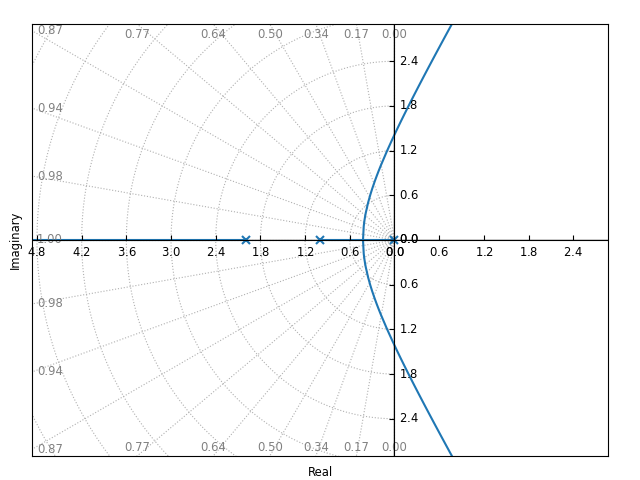
\includegraphics[scale=0.8]{../figures/rlocus/1320.png}
	\end{center}
	potremmo chiederci il valore del punto di intersezione fra i due rami.
	Ricordiamo allora la regola (5), per cui le radici doppie soddisfano:
	$$
	\sum_{i = 1}^n \frac{1}{s_i - p_i} = \sum_{i = 1}^m \frac{1}{s_i - z_i}
	$$
	che in questo caso significa:
	$$
	\frac{1}{s} + \frac{1}{s + 1} + \frac{1}{s + 2} = 0 \implies (s + 1) (s + 2) + s (s + 2) + s (s + 1) = 3s^2 + 6s + 2 = 0
	$$
	da cui le soluzioni:
	$$
		r_1 = \frac{-6 - \sqrt{12}}{6} \approx -1.577, \quad r_2 = \frac{-6 + \sqrt{12}}{6} \approx -0.4226
	$$
	dal grafico, si nota che il punto che cerchiamo dovrà essere compreso fra $-1$ e $0$, per cui prendiamo la seconda soluzione.

		\par\medskip
		\noindent
		\textbf{\sffamily{Esempio 3}}

		Prendiamo il caso di avere 2 poli coincidenti ed uno zero finito.
		In questo caso il luogo delle radici è una circonferenza centrata sullo zero.
		Questo si verifica dalla condizione di fase:
		$$
		\alpha - 2 \beta = - \pi \pm 2 h \pi
		$$
		Vogliamo dimostrare che questo vale su qualsiasi punto di una circonferenza centrata sullo zero e di raggio uguale alla differenza fra poli e zeri.
		Per questo prendiamo il disegno:
		\begin{center}
			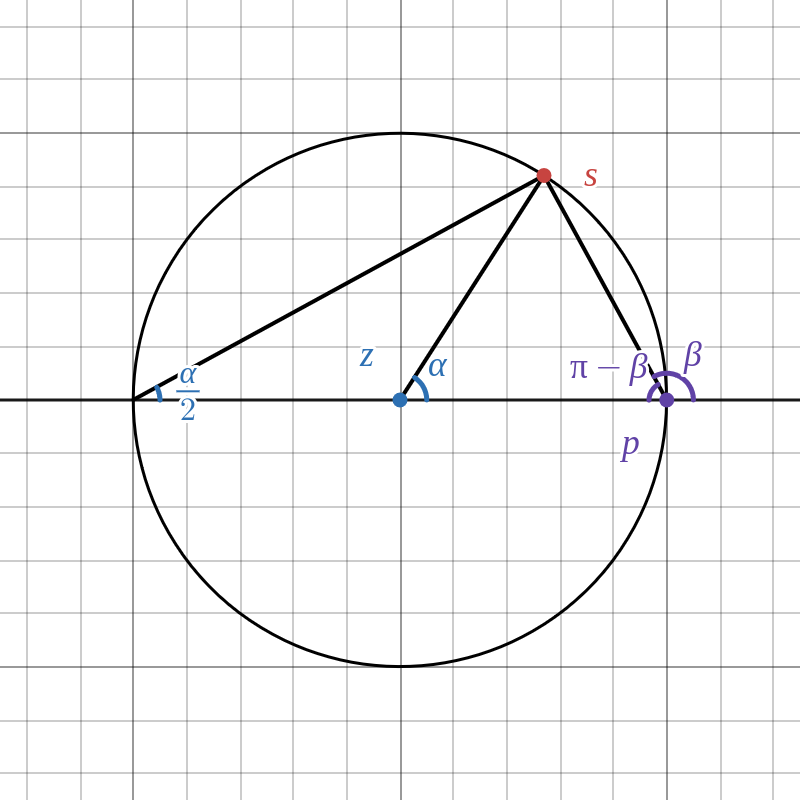
\includegraphics[scale=0.28]{../figures/rlocus_circ.png}
		\end{center}
		Osservando gli angoli si nota che deve valere:
		$$
		\frac{\alpha}{2} + (\pi - \beta) = \frac{\pi}{2} \, \Rightarrow \, \frac{\alpha}{2} - \beta = \frac{\pi}{2} - \pi \, \Rightarrow \, \alpha - 2 \beta = -\pi
		$$
		cioè la relazione, vera per ogni punto $s$ sulla circonferenza cercata, è equivalente alla condizione di fase per $h = 0$.

	\newpage

		Avremo quindi che i due poli, se sono reali, sono obbligatoriamente sovrapposti e tracciano il luogo:
	\begin{center}
		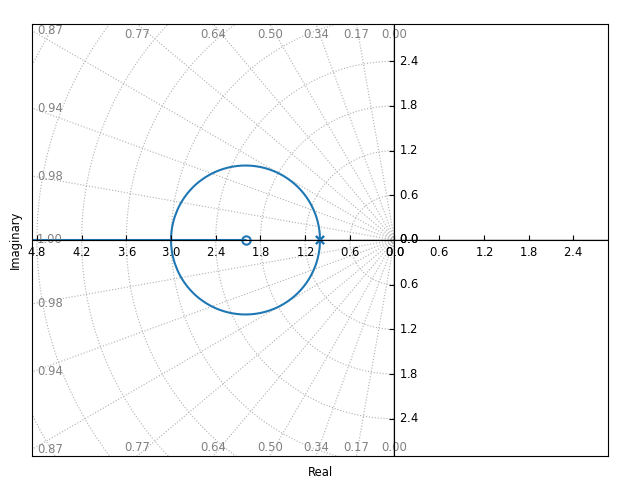
\includegraphics[scale=0.8]{../figures/rlocus/circ_full.png}
	\end{center}

	Il risultato si generalizza a funzioni di trasferimento qualsiasi con 2 poli complessi coniugati e uno zero finito.
	In questo caso il luogo è sempre una circonferenza vincolata sullo zero, dove i poli ne vincolano gli estremi:
	\begin{center}
		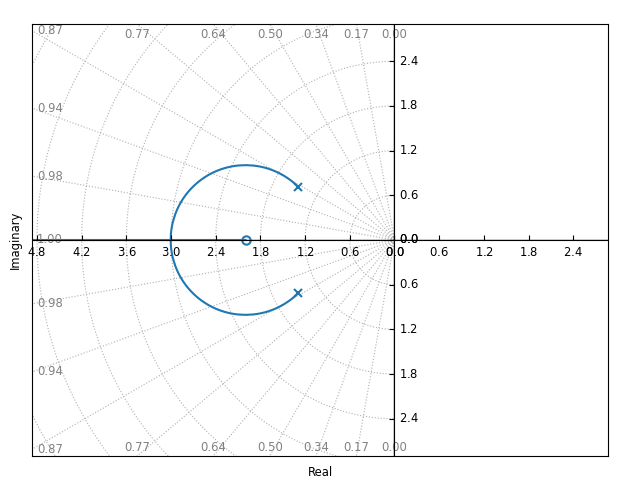
\includegraphics[scale=0.8]{../figures/rlocus/circ_cut.png}
	\end{center}

	\item[7.] La regola (7) riguarda gli angoli di partenza dei rami uscenti dai poli.
		Per ricavare una regola generale riprendiamo la condizione di fase:
		\[
			\begin{cases}
				\angle n(s) - \angle d(s) = -\pi \pm 2 h \pi, \quad K > 0 \\
				\angle n(s) - \angle d(s) = \pm 2 h \pi, \quad K < 0
			\end{cases}
		\]
		E notiamo che preso un polo particolare in $p^*$, ad esempio riguardo al luogo diretto, si avrà che l'angolo di uscita $\phi^*$ è:
		$$
		\angle n(s) - \angle d^*(s) \Big|_{s = p^*} - \phi^* = -\pi \implies \phi^* = \pi + \angle n(s) - \angle d^*(s) \Big|_{s = p^*}
		$$
		dove $d^*(s)$ è il denominatore rimosso il polo $p^*$ preso in considerazione.

		Potremo quindi usare questa formula generale per calcolare l'angolo di uscita dei rami dai poli.
		Da questo ricaviamo fra l'altro che i rami uscenti dai poli con molteplicità $> 1$ dividono il piano in parti equiangole e simmetriche rispetto all'asse reale.
		Infine, nessuno ci nega di applicare la stessa legge agli angoli di arrivo negli zeri (quindi di capire gli angoli finali dei rami che terminano \textit{al finito}).
		Vedremo questa situazione particolare nella regola (8).

		\par\medskip
		\noindent
		\textbf{\sffamily{Esempio}}

		Calcoliamo gli angoli di partenza dai poli della funzione di trasferimento:
		$$
		G(s) = \frac{s + 5}{s (s^2 + 6s + 109)}
		$$
		
		Partiamo col trovare i poli, di cui il polo banale $p_1 = 0$ e i poli complessi coniugati:
		$$
		p_{2, 3} = \frac{-6 \pm \sqrt{400}}{2} = -3 \pm 10i
		$$
		
		Abbiamo quindi i poli:
		$$
			p_1 = 0, \quad p_2 = -3 + 10 i, \quad p_3 = -3 - 10 i
		$$
		e la funzione di trasferimento fattorizzata:
		$$
		G(s) = \frac{s + 5}{s(s + 3 - 10i)(s + 3 + 10i)}
		$$

		Calcoliamo allora gli angoli veri e propri per ogni polo, applicando la legge appena trovata:
		\begin{itemize}
			\item Per il polo $p_1$ si ha cancellazione dei termini complessi:
		$$
		\phi_1 = \pi + \angle n(s) - \angle d^1(s) \Big|_{s = 0} = \pi + \angle 5 - \angle(3 - 10i) - \angle (3 + 10 i) =180^\circ
		$$
		e quindi il ramo è diretto a sinistra nell'asse reale, come ci aspettavamo dalla regola (4). 
	\item Per il polo $p_2$ prendiamo: 
		$$
		\phi_2 = \pi + \angle n(s) - \angle d^2(s) \Big|_{s = -3 + 10i} = \pi + \angle (-2 + 10i) - \angle (-3 + 10i) - \angle 20 i
		$$
		$$
		= 180^\circ + 78.7^\circ - 106.7^\circ - 90^\circ = 62^\circ
		$$
	\item Per il polo $p_3$ ci aspettiamo di trovare l'opposto di $\phi_2$, in quanto dalla regola (5) il luogo dovrà essere simmetrico rispetto all'asse reale.
		Facciamo comunqe il calcolo esplicito per completezza:
		$$
		\phi_3 = \pi + \angle n(s) - \angle d^3(s) \Big|_{s = -3 - 10i} = \pi + \angle (2 - 10i) - \angle (-3 - 10i) - \angle -20 i
		$$
		$$
		= 180^\circ - 78.7^\circ + 106.7^\circ + 90^\circ = -62^\circ
		$$
		che conferma quanto ci aspettavamo.
		\end{itemize}

		Vediamo quindi il grafico del luogo diretto:
		\begin{center}
			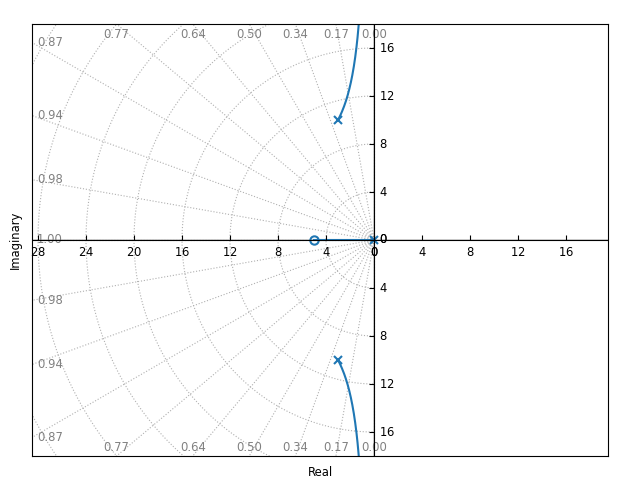
\includegraphics[scale=0.8]{../figures/rlocus/15_151090.png}
		\end{center}
\end{enumerate}

\end{document}
